%%%%%%%%%%%%%%%%%%%%%%%%%%%%%%%%%%%%%%%%%
% Beamer Presentation
% LaTeX Template
% Version 2.0 (March 8, 2022)
%
% This template originates from:
% https://www.LaTeXTemplates.com
%
% Author:
% Vel (vel@latextemplates.com)
%
% License:
% CC BY-NC-SA 4.0 (https://creativecommons.org/licenses/by-nc-sa/4.0/)
%
%%%%%%%%%%%%%%%%%%%%%%%%%%%%%%%%%%%%%%%%%

%----------------------------------------------------------------------------------------
%	PACKAGES AND OTHER DOCUMENT CONFIGURATIONS
%----------------------------------------------------------------------------------------

\documentclass[
	11pt, % Set the default font size, options include: 8pt, 9pt, 10pt, 11pt, 12pt, 14pt, 17pt, 20pt
	%t, % Uncomment to vertically align all slide content to the top of the slide, rather than the default centered
	%aspectratio=169, % Uncomment to set the aspect ratio to a 16:9 ratio which matches the aspect ratio of 1080p and 4K screens and projectors
]{beamer}

\graphicspath{{Images/}{./}} % Specifies where to look for included images (trailing slash required)

\usepackage{booktabs} % Allows the use of \toprule, \midrule and \bottomrule for better rules in tables

%----------------------------------------------------------------------------------------
%	SELECT LAYOUT THEME
%----------------------------------------------------------------------------------------

% Beamer comes with a number of default layout themes which change the colors and layouts of slides. Below is a list of all themes available, uncomment each in turn to see what they look like.

%\usetheme{default}
%\usetheme{AnnArbor}
%\usetheme{Antibes}
%\usetheme{Bergen}
%\usetheme{Berkeley}
%\usetheme{Berlin}
%\usetheme{Boadilla}
%\usetheme{CambridgeUS}
%\usetheme{Copenhagen}
%\usetheme{Darmstadt}
%\usetheme{Dresden}
%\usetheme{Frankfurt}
%\usetheme{Goettingen}
%\usetheme{Hannover}
%\usetheme{Ilmenau}
%\usetheme{JuanLesPins}
%\usetheme{Luebeck}
\usetheme{Madrid}
%\usetheme{Malmoe}
%\usetheme{Marburg}
%\usetheme{Montpellier}
%\usetheme{PaloAlto}
%\usetheme{Pittsburgh}
%\usetheme{Rochester}
%\usetheme{Singapore}
%\usetheme{Szeged}
%\usetheme{Warsaw}

%----------------------------------------------------------------------------------------
%	SELECT COLOR THEME
%----------------------------------------------------------------------------------------

% Beamer comes with a number of color themes that can be applied to any layout theme to change its colors. Uncomment each of these in turn to see how they change the colors of your selected layout theme.

%\usecolortheme{albatross}
%\usecolortheme{beaver}
%\usecolortheme{beetle}
%\usecolortheme{crane}
%\usecolortheme{dolphin}
%\usecolortheme{dove}
%\usecolortheme{fly}
%\usecolortheme{lily}
%\usecolortheme{monarca}
%\usecolortheme{seagull}
%\usecolortheme{seahorse}
%\usecolortheme{spruce}
%\usecolortheme{whale}
%\usecolortheme{wolverine}

%----------------------------------------------------------------------------------------
%	SELECT FONT THEME & FONTS
%----------------------------------------------------------------------------------------

% Beamer comes with several font themes to easily change the fonts used in various parts of the presentation. Review the comments beside each one to decide if you would like to use it. Note that additional options can be specified for several of these font themes, consult the beamer documentation for more information.

\usefonttheme{default} % Typeset using the default sans serif font
%\usefonttheme{serif} % Typeset using the default serif font (make sure a sans font isn't being set as the default font if you use this option!)
%\usefonttheme{structurebold} % Typeset important structure text (titles, headlines, footlines, sidebar, etc) in bold
%\usefonttheme{structureitalicserif} % Typeset important structure text (titles, headlines, footlines, sidebar, etc) in italic serif
%\usefonttheme{structuresmallcapsserif} % Typeset important structure text (titles, headlines, footlines, sidebar, etc) in small caps serif

%------------------------------------------------

%\usepackage{mathptmx} % Use the Times font for serif text
\usepackage{palatino} % Use the Palatino font for serif text

%\usepackage{helvet} % Use the Helvetica font for sans serif text
\usepackage[default]{opensans} % Use the Open Sans font for sans serif text
%\usepackage[default]{FiraSans} % Use the Fira Sans font for sans serif text
%\usepackage[default]{lato} % Use the Lato font for sans serif text


%----------------------------------------------------------------------------------------
%	SELECT INNER THEME
%----------------------------------------------------------------------------------------

% Inner themes change the styling of internal slide elements, for example: bullet points, blocks, bibliography entries, title pages, theorems, etc. Uncomment each theme in turn to see what changes it makes to your presentation.

%\useinnertheme{default}
\useinnertheme{circles}
%\useinnertheme{rectangles}
%\useinnertheme{rounded}
%\useinnertheme{inmargin}

%----------------------------------------------------------------------------------------
%	SELECT OUTER THEME
%----------------------------------------------------------------------------------------

% Outer themes change the overall layout of slides, such as: header and footer lines, sidebars and slide titles. Uncomment each theme in turn to see what changes it makes to your presentation.

%\useoutertheme{default}
%\useoutertheme{infolines}
%\useoutertheme{miniframes}
%\useoutertheme{smoothbars}
%\useoutertheme{sidebar}
%\useoutertheme{split}
%\useoutertheme{shadow}
%\useoutertheme{tree}
%\useoutertheme{smoothtree}

%\setbeamertemplate{footline} % Uncomment this line to remove the footer line in all slides
%\setbeamertemplate{footline}[page number] % Uncomment this line to replace the footer line in all slides with a simple slide count

%\setbeamertemplate{navigation symbols}{} % Uncomment this line to remove the navigation symbols from the bottom of all slides

%----------------------------------------------------------------------------------------
%	PRESENTATION INFORMATION
%----------------------------------------------------------------------------------------

\title[ECM3420 CA]{Predicting Activity Based on Device Accelerometer Data} % The short title in the optional parameter appears at the bottom of every slide, the full title in the main parameter is only on the title page

\subtitle{ECM3420 Coursework} % Presentation subtitle, remove this command if a subtitle isn't required

\author[Ethan Hofton]{Ethan Hofton} % Presenter name(s), the optional parameter can contain a shortened version to appear on the bottom of every slide, while the main parameter will appear on the title slide

\institute[UofE]{University of Exeter \\ \smallskip \textit{eh736@exeter.ac.uk}} % Your institution, the optional parameter can be used for the institution shorthand and will appear on the bottom of every slide after author names, while the required parameter is used on the title slide and can include your email address or additional information on separate lines

\date[\today]{\today} % Presentation date or conference/meeting name, the optional parameter can contain a shortened version to appear on the bottom of every slide, while the required parameter value is output to the title slide

%----------------------------------------------------------------------------------------

\begin{document}

%----------------------------------------------------------------------------------------
%	TITLE SLIDE
%----------------------------------------------------------------------------------------

\begin{frame}
	\titlepage % Output the title slide, automatically created using the text entered in the PRESENTATION INFORMATION block above
\end{frame}

%----------------------------------------------------------------------------------------
%	TABLE OF CONTENTS SLIDE
%----------------------------------------------------------------------------------------

% The table of contents outputs the sections and subsections that appear in your presentation, specified with the standard \section and \subsection commands. You may either display all sections and subsections on one slide with \tableofcontents, or display each section at a time on subsequent slides with \tableofcontents[pausesections]. The latter is useful if you want to step through each section and mention what you will discuss.

% \begin{frame}
% 	\frametitle{Presentation Overview} % Slide title, remove this command for no title
	
% 	\tableofcontents % Output the table of contents (all sections on one slide)
% 	%\tableofcontents[pausesections] % Output the table of contents (break sections up across separate slides)
% \end{frame}

%----------------------------------------------------------------------------------------
%	PRESENTATION BODY SLIDES
%----------------------------------------------------------------------------------------

\section{Text Examples} % Sections are added in order to organize your presentation into discrete blocks, all sections and subsections are automatically output to the table of contents as an overview of the talk but NOT output in the presentation as separate slides

%------------------------------------------------

\subsection{Research Question}

\begin{frame}
	\frametitle{Research Question}
	
	Can the type of activity people are doing be inferred from device accelerometer data?

    \bigskip
		Why should anyone care about this?

    \begin{itemize}
        \item Health and fitness monitoring
        \item Safty and wellbeing
        \item Environmental monitoring
    \end{itemize}

    \bigskip

    Real world applications:
    \begin{itemize}
        \item Fitness and health trackers
        \item Emergency response applications
    \end{itemize}
\end{frame}

%------------------------------------------------

\section{Dataset}

\begin{frame}
	\frametitle{The Dataset \cite{motionsense}}

    \begin{columns}
        \column{0.5\textwidth}
            \begin{itemize}
            \item attitude (roll, pitch, yaw)
            \item gravity (x, y, z)
            \item rotationRate (x, y, z)
            \item userAcceleration (x, y, z)
            \item Time series data
            \end{itemize}

        \column{0.5\textwidth}
            \begin{itemize}
                \item 24 participants
                \item 6 activities (walking, jogging, upstairs, downstairs, sitting, standing)
                \item 15 trials, 9 long (3 mins each), 6 short (30 secs each)
                \item 50Hz sampling rate
            \end{itemize}
    \end{columns}
	
    \begin{figure}[]
        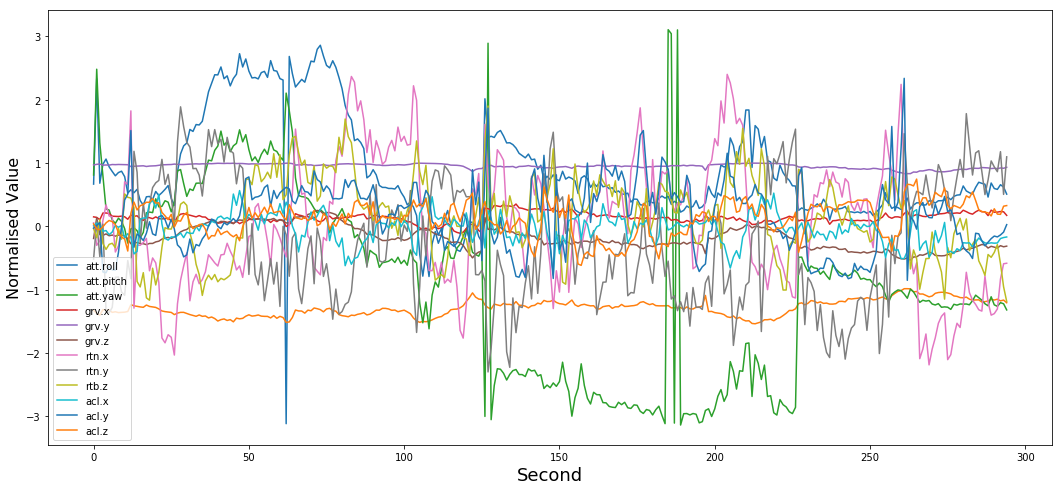
\includegraphics[width=0.5\linewidth]{dataset.png}
        \caption{A sample from the dataset \cite{dataset:online} }
    \end{figure}
\end{frame}

\begin{frame}
    \frametitle{Machine Learning Methods}

    \begin{block}{Predicting Activity}
        \begin{itemize}
            \item Classification Problem
            \item Supervised Learning
            \item Multi-Class (DWS, UPS, SIT, STD, WLK, JOG)
        \end{itemize}
    \end{block}

    \bigskip

    \begin{block}{Feature Selection}
        \begin{itemize}
            \item PCA for dimensionality reduction
            \item Unsupervised Learning
        \end{itemize}
    \end{block}
\end{frame}

\begin{frame}
    \frametitle{Data Preprocessing}
    \framesubtitle{Data Cleaning}

    \begin{block}{Data Cleaning}
        \begin{itemize}
            \item Data is already clean
            \item The data can be split into train test sets
            \begin{itemize}
                \item The long trails (1-9) are used for training
                \item The short trails (10-15) are used for testing
                \item For NN models, the train data will be split 80/20 into train and validation sets 
            \end{itemize}
        \end{itemize}
    \end{block}

    \begin{block}{Feature Engeneering}
        User acceleration and gravity are combined to get the total acceleration. This reduces the dimensions of the data.

        The norm of the total acceleration is also calculated. This is used as a feature for the NN models
    \end{block}
\end{frame}

\begin{frame}
    \frametitle{Data Preprocessing}
    \framesubtitle{Dimentsionality Reduction}

    Combine gravity and user acceleration and remove the original columns. Is this a good idea?

    \begin{columns}
        \column{0.5\textwidth}
        \begin{figure}[]
            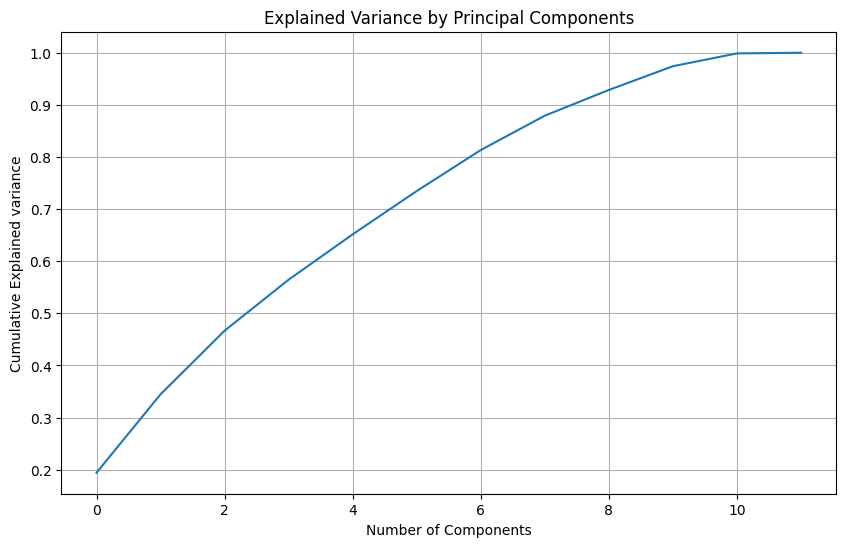
\includegraphics[width=0.9\linewidth]{pca_before.png}
            \caption{PCA on the data}
        \end{figure}

        \column{0.5\textwidth}
        \begin{figure}
            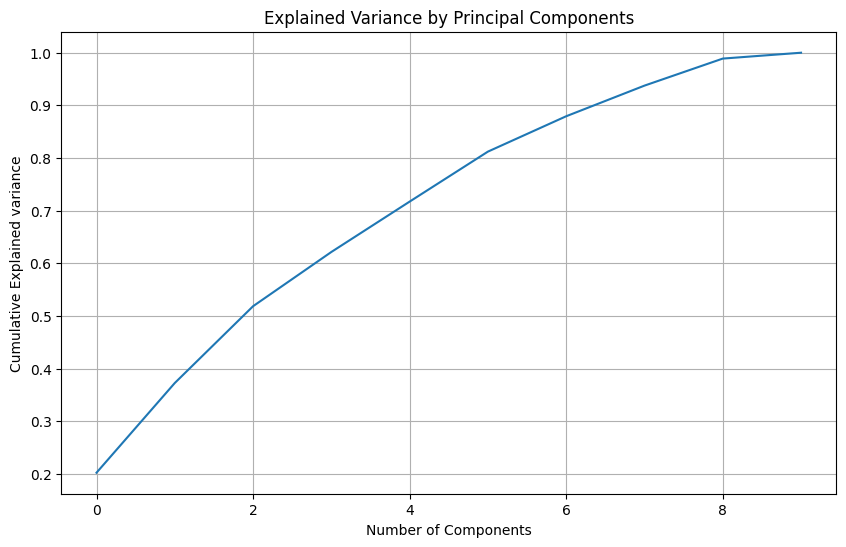
\includegraphics[width=0.9\linewidth]{pca_after.png}
            \caption{PCA on the data with gravity and user acceleration combined}
        \end{figure}
    \end{columns}
        
\end{frame}


\begin{frame}
    \frametitle{Data Analysis}
    \framesubtitle{Models}
    
    \begin{itemize}
        \item Decision Tree
        \item Random Forest
        \item Neural Network
        \item Convolutional Neural Network
        \item Simple Recurrent Neural Network
        \item Long Short Term Memory
    \end{itemize}
\end{frame}

\begin{frame}
    \frametitle{Data Analysis}
    \framesubtitle{Model Architecture}

    \begin{columns}
        \column{0.5\textwidth}
        \begin{block}{Decision Tree}
            Standard decision tree with no hyperparameter tuning
        \end{block}

        \column{0.45\textwidth}
        \begin{block}{Random Forest}
            10 estimators
        \end{block}
    \end{columns}

    \begin{block}{Neural Network}
        \begin{itemize}
            \item 10 neuron input layer
            \item 1 hidden layer with 64 neurons, relu activation
            \item 1 hidden layer with 32 neurons, relu activation
            \item 1 output layer with 6 neurons, softmax activation
        \end{itemize}
    \end{block}

\end{frame}

\begin{frame}
    \frametitle{Data Analysis}
    \framesubtitle{Early Results}
    
	\begin{table}
		\begin{tabular}{l l l l l l l l}
			\toprule
			\textbf{Model} & \textbf{DWS} & \textbf{UPS} & \textbf{SIT} & \textbf{STD} & \textbf{WLK} & \textbf{JOG} & Total \\
			\midrule
			Decision Tree & 48.1 & 51.7 & 94.7 & 90.3 & 59.2 & 60.5 & 76.7 \\
            Random Forest & 62.7 & 59.1 & 94.9 & 92.6 & 70.4 & 71.7 & 82.2 \\
            Neural Network & 49.4 & 46.4 & 89.4 & 92.2 & 76.2 & 70.0 & 79.4 \\
			\bottomrule
		\end{tabular}
		\caption{Results of the models on the test dataset}
	\end{table}

    \begin{block}{Results}
        These results could be better. The models do not take into account the time series nature of the data.
    \end{block}
    
\end{frame}

%------------------------------------------------


\begin{frame}
    \frametitle{Data Preprocessing}
    \framesubtitle{Time Series Data}

    \begin{block}{Windowing}
        The input data is slid over in windows of size 150 (3 seconds). The stride of the window is 10 (0.2 seconds). The resulting window is a 150x10 matrix. This data can be passed to a neural network model suited to time series/2 dimensional data like CNN, RNN.
    \end{block}

    \begin{block}{Rolling Features}
        Rolling features involves calculating a rolling mean, standard deviation and median for each feature of the data. This allows the data to be passed to a model that is not suited to time series data like a decision tree or random forest without losing the time series nature of the data.
    \end{block}
\end{frame}

\begin{frame}
    \frametitle{Data Analysis}
    \framesubtitle{Rolling Features}

    \begin{table}
		\begin{tabular}{l l l l l l l l}
			\toprule
			\textbf{Model} & \textbf{DWS} & \textbf{UPS} & \textbf{SIT} & \textbf{STD} & \textbf{WLK} & \textbf{JOG} & Total \\
			\midrule
			Decision Tree & 90.1 & 88.1 & 91.6 & 99.7 & 85.4 & 89.3 & 91.9 \\
            Random Forest & 98.6 & 94.6 & 99.9 & 96.3 & 90.4 & 96.0 & 96.3 \\
            Neural Network & 94.6 & 89.8 & 90.5 & 95.6 & 91.5 & 96.4 & 92.7 \\
			\bottomrule
		\end{tabular}
		\caption{Results of models on the rolling features dataset}
	\end{table}
\end{frame}


\begin{frame}
    \frametitle{Data Analysis}
    \framesubtitle{Rolling Feature Results}

    \begin{figure}
        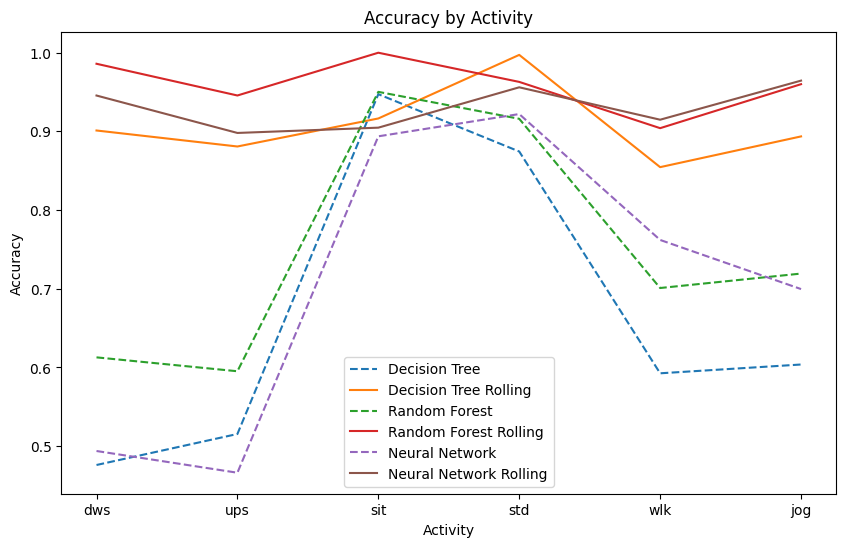
\includegraphics[width=0.6\linewidth]{rolling_before_after.png}
        \caption{Results before and after rolling features are applied}
    \end{figure}

    \begin{itemize}
        \item Time series data is not important for sitting and standing (no movement)
    \end{itemize}

\end{frame}

\begin{frame}
    \frametitle{Data Analysis}
    \framesubtitle{Confusion Matrix}

    \begin{columns}
        \column{0.5\textwidth}
        \begin{figure}[]
            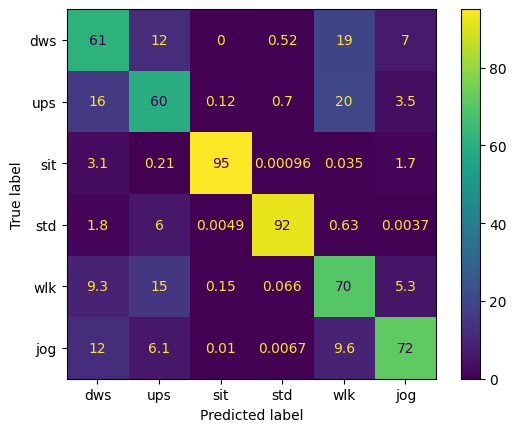
\includegraphics[width=0.9\linewidth]{cm_rtc_before.png}
            \caption{Random Forest confusion matrix before rolling features}
        \end{figure}

        \column{0.5\textwidth}
        \begin{figure}
            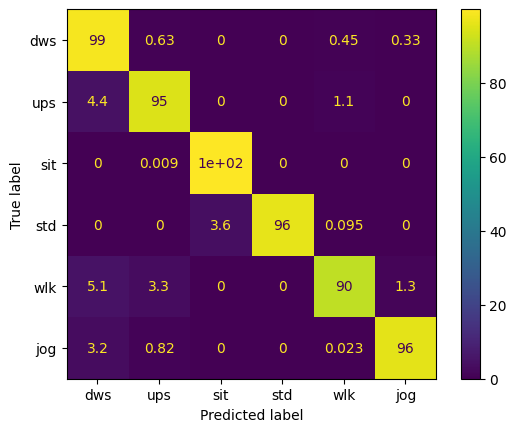
\includegraphics[width=0.9\linewidth]{cm_rtc_after.png}
            \caption{Random Forest confusion matrix after rolling features}
        \end{figure}
    \end{columns}
\end{frame}

\begin{frame}
    \frametitle{Model Architecture}

    \begin{block}{CNN Architecture}
        \begin{itemize}
            \item 1D Convolutional Layer, 64 filters, 3x3 kernal
            \item Max Pooling Layer
            \item Dropout layer, 0.2 dropout rate
            \item 1D Convolutional Layer, 32 filters, 3x3 kernal
            \item Max Pooling Layer
            \item Dropout layer, 0.2 dropout rate
            \item Flatten Layer
            \item Dense layer, 64 neurons, L2 regularization, relu activation
            \item Dense layer, 32 neurons, L2 regularization, relu activation
            \item 6 neuron output layer, softmax activation
        \end{itemize}
    \end{block}

    LSTM and RNN followed the same Architecture but with a single LSTM or RNN layer instead of the CNN layers

\end{frame}

\begin{frame}
    \frametitle{Data Analysis}
    \framesubtitle{Sliding Window Results}


    \begin{table}
		\begin{tabular}{l l l l l l l l}
			\toprule
			\textbf{Model} & \textbf{DWS} & \textbf{UPS} & \textbf{SIT} & \textbf{STD} & \textbf{WLK} & \textbf{JOG} & Total \\
			\midrule
			CNN & 95.3 & 90.4 & 95.2 & 95.9 & 92.9 & 97.8 & 94.7 \\
            LSTM & 96.8 & 92.7 & 95.3 & 92.4 & 92.9 & 95.3 & 94.0 \\
            RNN & 94.0 & 91.7 & 95.3 & 94.6 & 93.7 & 89.4 & 93.9 \\
			\bottomrule
		\end{tabular}
		\caption{Results of models on the windowing features dataset}
	\end{table}

\end{frame}

\begin{frame}

    \frametitle{Data Analysis}
    \framesubtitle{Adjusting the side of the window}

    \begin{figure}
        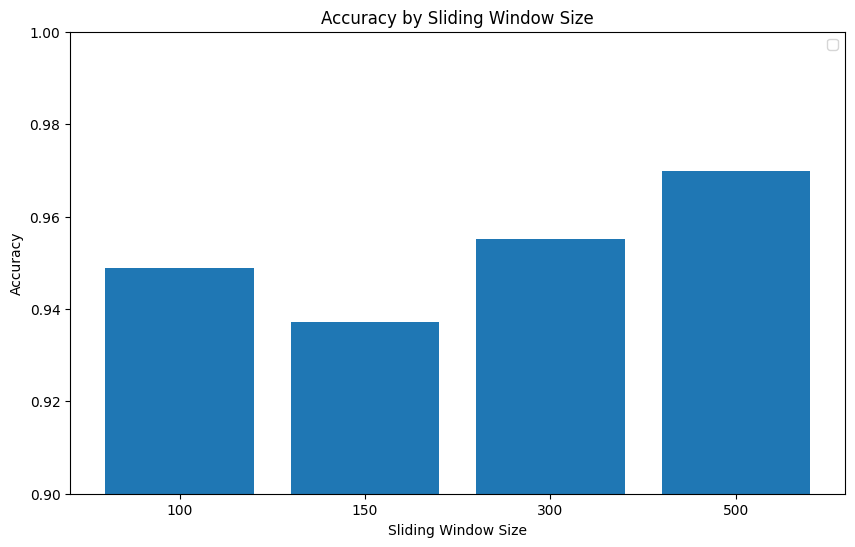
\includegraphics[width=0.6\linewidth]{window_size.png}
        \caption{Results of the CNN model with different window sizes}
    \end{figure}
    
\end{frame}

\begin{frame}

    \frametitle{Data Analysis}
    \framesubtitle{2s vs 10s Windows}

    \begin{columns}        
        \column{0.5\textwidth}
        \begin{figure}
            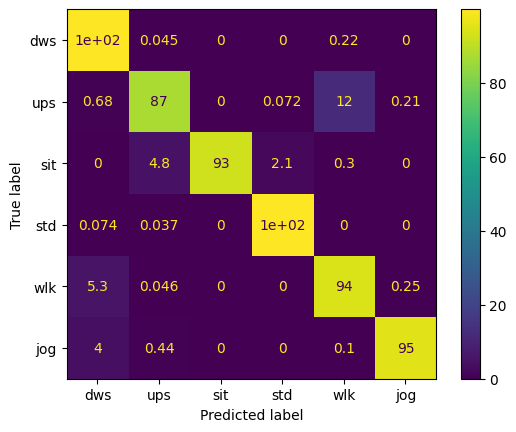
\includegraphics[width=0.9\linewidth]{cm_sliding_100.png}
            \caption{CNN confusion matrix with 2s windows}
        \end{figure}

        \column{0.5\textwidth}
        \begin{figure}
            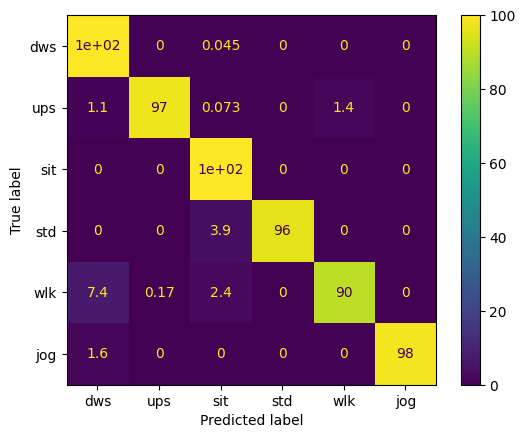
\includegraphics[width=0.9\linewidth]{cm_sliding_500.png}
            \caption{CNN confusion matrix with 10s windows}
        \end{figure}
    \end{columns}
    
\end{frame}

\begin{frame}

    \frametitle{Data Analysis}
    \framesubtitle{Rolling Features vs Windowing}

    \begin{columns}        
        \column{0.5\textwidth}
        \begin{figure}
            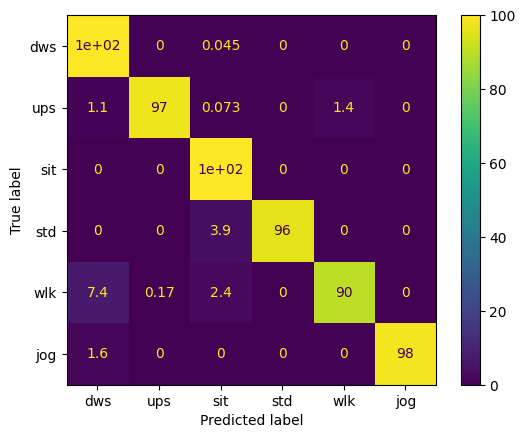
\includegraphics[width=0.9\linewidth]{cm_sliding_500.png}
            \caption{CNN confusion matrix with 10s windows}
        \end{figure}

        \column{0.5\textwidth}
        \begin{figure}
            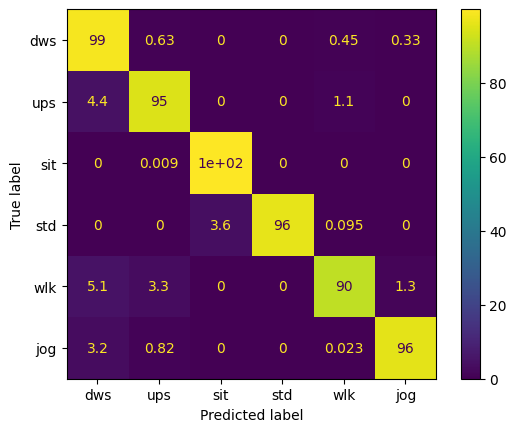
\includegraphics[width=0.9\linewidth]{cm_rtc_after.png}
            \caption{CNN confusion matrix Random Forest with rolling features}
        \end{figure}
    \end{columns}
    
\end{frame}

\begin{frame}
    \frametitle{Conclusion}    
    \framesubtitle{Results Overview}

    \begin{itemize}
        \item Random Forest with rolling features achived 96.3\% accuracy
        \item CNN with 10s windows achieved 97\% accuracy
        \item CNN training time was approximately 13 minuets
        \item Random Forest training time was approximately 1.5 minuets
    \end{itemize}

\end{frame}

\begin{frame}{title}
    \frametitle{Concluding Remarks}

    \begin{block}{Results}
        \begin{itemize}
            \item Time series data is important for activities with movement
            \item Data with time series features performs better than data without
            \item Windowing and rolling features are both good ways to deal with time series data
            \item Windowing lead to better results than rolling features
            \item Windowing is more computationally expensive than rolling features
            \item Rolling features were quicker to train and predict than windowing
        \end{itemize}
    \end{block}

\end{frame}

\begin{frame}
    \frametitle{Limitations}

    \begin{block}{The Data}
    \begin{itemize}
        \item The dataset is small
        \item The dataset is not diverse
        \item The dataset is not real world
    \end{itemize}
    \end{block}

    \begin{block}{The Models}
    \begin{itemize}
        \item Overfitting
        \item Computational cost 
        \item Black box
    \end{itemize}
    \end{block}

\end{frame}

\begin{frame}[allowframebreaks] % Use [allowframebreaks] to allow automatic splitting across slides if the content is too long
	\frametitle{References}
	
    \begin{thebibliography}{9}
        \footnotesize % Reduce the font size in the bibliography

        \bibitem{motionsense}
        Mohammad Malekzadeh, Richard G. Clegg, Andrea Cavallaro, and Hamed Haddadi.
        \textit{Mobile Sensor Data Anonymization}.
        In \textit{Proceedings of the International Conference on Internet of Things Design and Implementation (IoTDI '19)}, 
        Montreal, Quebec, Canada, 2019. 
        ISBN: 978-1-4503-6283-2.
        Pages 49--58.
        \url{http://doi.acm.org/10.1145/3302505.3310068}
        
        \bibitem{dataset:online}
        \textit{motion-sense/materials/desc.png at master · mmalekzadeh/motion-sense}.
        \url{https://github.com/mmalekzadeh/motion-sense/blob/master/materials/desc.png}.
        Accessed on 12/02/2023.
        
    \end{thebibliography}
\end{frame}

\end{document} 